The equation \eqref{eq:solutions/1/19/Q} can be written as,
\begin{align}
y^2-3x+2 = 0
\end{align}
Comparing it with standard equation,
\begin{align}
ax^2+2bxy+cy^2+2dx+2ey+f = 0
\end{align}
$\therefore$ a = b = e = 0, d = $\frac{-3}{2}$, c = 1, f = 2.
\begin{align}
\therefore \vec{V} = \myvec{a&b\\b&c} = \myvec{0&0\\0&1}
\end{align} 
\begin{align}
\therefore\vec{u} = \myvec{d\\e} = \myvec{\frac{-3}{2}\\0}\label{eq:solutions/1/19/u}
\end{align}
\begin{align}
 \mbox{ Now,} \mydet{V} = \mydet{0&0\\0&1} = 0
\end{align}
$\implies$ that the curve is a parabola. Now, finding the eigen values corresponding to the $\vec{V}$,
\begin{align}
\mydet{\vec{V}-\lambda\vec{I}} = 0
\end{align}
\begin{align}
\mydet{-\lambda&0\\0&1-\lambda} = 0
\end{align}
\begin{align}
\implies \lambda = 0,1.
\end{align}
Calculating the eigenvectors corresponding to $\lambda = 0,1$ respectively,
\begin{align}
\vec{V}\vec{x} = \lambda\vec{x}
\end{align}
\begin{align}
\myvec{0&0\\0&1}\vec{x} = 0 \implies \vec{p_1} = \myvec{1\\0}
\end{align}
\begin{align}
\myvec{0&0\\0&1}\vec{x} = \vec{x} \implies \vec{p_2} = \myvec{0\\1}
\end{align}
Now by eigen decomposition on $\vec{V}$,
\begin{align}
\vec{V} = \vec{PDP^T}
\label{eq:solutions/1/19/V}
\end{align}
\begin{align}
\mbox{where,} \vec{P} = \myvec{\vec{p_1} \vec{p_2}} = \myvec{1&0\\0&1}
\end{align}
\begin{align}
\vec{D} = \myvec{\lambda_1&0\\0&\lambda_2} = \myvec{0&0\\0&1}
\end{align}
Hence equation \eqref{eq:solutions/1/19/V} becomes,
\begin{align}
\vec{V} = \myvec{1&0\\0&1}\myvec{0&0\\0&1}\myvec{1&0\\0&1}
\end{align}
\begin{align}
\vec{V} = \myvec{0&0\\0&1}
\end{align}
Now the tangent to parabola is parallel to the line equation \eqref{eq:solutions/1/19/P}, Hence the direction vectors ($\vec{m}$) and normal ($\vec{n}$)  vectors are,
\begin{align}
\vec{m} = \myvec{1\\-2}\\
\vec{n} = \myvec{2\\1}\label{eq:solutions/1/19/n}
\end{align} 
Now, the equation for the point of contact for the parabola is given as,
\begin{align}
\myvec{\vec{u}^T+\kappa\vec{n}^T\\\vec{V}}\vec{q} = \myvec{-f\\\kappa\vec{n}-\vec{u}}\label{eq:solutions/1/19/contact}\\
\mbox{where, } \kappa = \frac{\vec{p_1}^T\vec{u}}{\vec{p_1}^T\vec{n}} = \frac{-3}{4} \label{eq:solutions/1/19/k}
\end{align}
Hence substituting the values of \eqref{eq:solutions/1/19/k}, \eqref{eq:solutions/1/19/n}, \eqref{eq:solutions/1/19/V} and \eqref{eq:solutions/1/19/u} in equation \eqref{eq:solutions/1/19/contact} we get,
\begin{align}
\myvec{-3&\frac{-3}{4}\\0&0\\0&1}\vec{q} = \myvec{-2\\0\\\frac{-3}{4}}
\label{eq:solutions/1/19/solve_q}
\end{align}
Solving for $\vec{q}$ by removing the zero row and representing \eqref{eq:solutions/1/19/solve_q} as augmented matrix and then converting the matrix to echelon form,
\begin{align}
\implies \myvec{-3&\frac{-3}{4}&-2\\0&1&\frac{-3}{4}} \xleftrightarrow[]{R_1\leftarrow\brak{\frac{-R_1}{3}}} \myvec{1&\frac{1}{4}&\frac{2}{3}\\0&1&\frac{-3}{4}}
\end{align}
\begin{align}
\xleftrightarrow[]{R_1\leftarrow R_1-\frac{1}{4}R_2} \myvec{1&0&\frac{41}{48}\\0&1&\frac{-3}{4}}
\label{eq:solutions/1/19/q_value}
\end{align}
Hence from equation \eqref{eq:solutions/1/19/q_value} it can be concluded that the point of contact is,
\begin{align}
\vec{q} = \myvec{\frac{41}{48}\\\frac{-3}{4}}
\end{align}
Now $\vec{q}$ is a point on the tangent. Hence, the equation of the
line can be expressed as
\begin{align}
\vec{n}^T\vec{x} = c
\label{eq:solutions/1/19/tangent}
\end{align}
where c is,
\begin{align}
 c = \vec{n}^T\vec{q} = \myvec{2&1}\myvec{\frac{41}{48}\\\frac{-3}{4}} = \frac{23}{24} 
 \label{eq:solutions/1/19/const}
\end{align}
Hence equation of tangent to the curve \eqref{eq:solutions/1/19/Q} parallel to \eqref{eq:solutions/1/19/P} is given by substituting the value of c and $\vec{n}$ from equation \eqref{eq:solutions/1/19/const} and \eqref{eq:solutions/1/19/n} respectively to the equation \eqref{eq:solutions/1/19/tangent},
\begin{align}
\implies\myvec{2&1}\vec{x} = \frac{23}{24} 
\end{align}
Figure \ref{eq:solutions/1/19/Figure_1} verifies that the $\myvec{2&1}\vec{x} = \frac{23}{24}$ is a tangent to parabola  $y=\sqrt{3x-2}$
\begin{figure}[ht!]
\centering
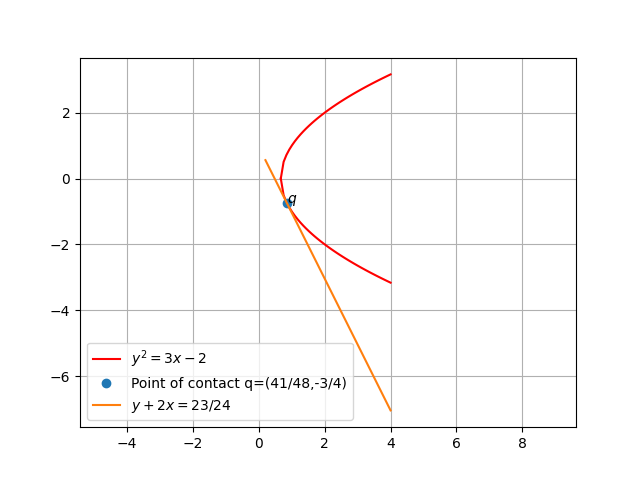
\includegraphics[width=\columnwidth]{./solutions/conics/1/19/Figure_1.png}
\caption{Tangent to parabola $y=\sqrt{3x-2}$}
\label{eq:solutions/1/19/Figure_1}
\end{figure}
